% ============================================================
%  CropGuard — Final SRS (Assignment 3)
%  Author : Protik Barua, ID 2110082
%  Course : Web Application And Internet
%  Instructor : Md. Abu Sayed
% ============================================================
\documentclass[12pt,a4paper]{article}

% ── packages ──────────────────────────────────────────────
\usepackage[margin=1in]{geometry}
\usepackage{newtxtext,newtxmath}
\usepackage{graphicx}
\usepackage{booktabs}
\usepackage{tabularx}
\usepackage{longtable}
\usepackage{enumitem}
\usepackage{hyperref}
\usepackage[table]{xcolor}
\usepackage{fancyhdr}
\usepackage{titlesec}
\usepackage{tocloft}
\usepackage{float}
\usepackage{amsmath}
\usepackage{tikz}
\usetikzlibrary{shapes,arrows.meta,positioning,fit,backgrounds,calc}

% ── colours ───────────────────────────────────────────────
\definecolor{cropgreen}{HTML}{2E7D32}
\definecolor{lightgreen}{HTML}{E8F5E9}
\definecolor{darkgray}{HTML}{333333}
\definecolor{medgray}{HTML}{666666}
\definecolor{accentblue}{HTML}{1565C0}
\definecolor{warnred}{HTML}{C62828}

% ── hyperlinks ────────────────────────────────────────────
\hypersetup{
    colorlinks=true,
    linkcolor=cropgreen,
    urlcolor=accentblue,
    citecolor=cropgreen
}

% ── header / footer ──────────────────────────────────────
\pagestyle{fancy}
\fancyhf{}
\fancyhead[L]{\small\textcolor{medgray}{Software Requirement Specification (SRS) For CropGuard}}
\fancyfoot[C]{\thepage}
\renewcommand{\headrulewidth}{0.4pt}

% ── section styling ──────────────────────────────────────
\titleformat{\section}
  {\Large\bfseries\color{cropgreen}}{\thesection}{1em}{}
\titleformat{\subsection}
  {\large\bfseries\color{darkgray}}{\thesubsection}{1em}{}
\titleformat{\subsubsection}
  {\normalsize\bfseries\color{medgray}}{\thesubsubsection}{1em}{}

% ── spacing ──────────────────────────────────────────────
\setlength{\parskip}{6pt}
\setlength{\parindent}{0pt}

% ── custom command for FR boxes ──────────────────────────
\newcommand{\frbox}[5]{%
  \begin{table}[H]
  \centering
  \begin{tabularx}{\textwidth}{|l|X|}
  \hline
  \rowcolor{lightgreen}
  \textbf{Requirement ID} & \textbf{#1} \\
  \hline
  \textbf{Primary Actor} & #2 \\
  \hline
  \textbf{Trigger} & #3 \\
  \hline
  \textbf{Description} & #4 \\
  \hline
  \rowcolor{lightgreen}
  \textbf{Acceptance Criteria} & #5 \\
  \hline
  \end{tabularx}
  \end{table}
}

% ══════════════════════════════════════════════════════════
\begin{document}

% ── title page ───────────────────────────────────────────
\begin{titlepage}
\centering
\vspace*{1.5cm}

{\Huge\bfseries\textcolor{cropgreen}{CropGuard}}\\[0.5cm]
{\Large A Smart Web-Based Crop Disease Detection and\\
Advisory System with AI-Powered Leaf Analysis\\
for Smallholder Farmers in Bangladesh}

\vspace{1.5cm}

{\large\textbf{Software Requirements Specification}}\\[0.3cm]
{\normalsize Final SRS }

\vspace{2cm}

\begin{tabular}{rl}
\textbf{Submitted to:} & Md. Abu Sayed \\
                         \\[0.8cm]
\textbf{Prepared by:}  & Protik Barua \\
                        & ID: 2110082 \\
                        & Course: Web Application And Internet \\[0.8cm]
\textbf{Department:}   & Computer Science and Engineering \\
                        & Independent University, Bangladesh \\[0.8cm]
\textbf{Date:}         & \today
\end{tabular}

\vfill

\end{titlepage}

% ── table of contents ────────────────────────────────────
\newpage
\tableofcontents
\newpage

% ══════════════════════════════════════════════════════════
%  1. EXECUTIVE SUMMARY
% ══════════════════════════════════════════════════════════
\section{Executive Summary}

This is the software requirements specification for CropGuard. CropGuard is an online system that assists smallholder farmers in rural Bangladesh to detect diseases in their crops by analysing the images of crop leaves. The inspiration for CropGuard is simple - in places such as Ukhia, Bancharampur and Comilla, farmers sometimes lose a substantial part of their crop due to failure to quickly identify the problem. They generally rely on their own knowledge or herbs and pesticide sellers.

CropGuard aims to change that. By uploading an image of a diseased leaf, a farmer is able to get a diagnosis and treatment suggestions (chemical, biological and cultural). CropGuard also has a database of 12 popular diseases affecting rice, potato, tomato and mango; and enables farmers to reach out to agricultural extension officers by phone, WhatsApp and email.

The big-picture objectives are straightforward:

\begin{itemize}[leftmargin=2em]
  \item Offer farmers a quick method to diagnose crop diseases, without having to wait days for a diagnosis.
  \item Recommend a treatment, including natural and chemical options, as farmers may not be able to afford pesticides.
  \item Keep a simple disease database which can be accessed even by less technically savvy users.
  \item Maintain an admin side disease database, user account database and the ability to send alerts regarding particular disease outbreaks.
\end{itemize}

This is a student project and has a short time constraint, so not all features (Bangla interface, offline mode, SMS) are implemented here. But the main diagnosis process, disease database and communication with experts are all working.

% ══════════════════════════════════════════════════════════
%  2. INTRODUCTION
% ══════════════════════════════════════════════════════════
\section{Introduction}

CropGuard is targeted at a particular group of users: small farmers in Bangladesh, who usually grow Boro rice, Aman paddy, potato, tomato and/or mangoes in less than 2 hectares of land. We have developed the system based on a survey of 5 farmers of Ukhiya, Bancharampur, Comilla and rural Dhaka and 15 research papers on crop disease detection and deep learning.

The internet has become more popular in rural Bangladesh. Our research shows 80\% of farmers have smartphones, which is great. But only 20\% have used any agriculture related app. Apparently, they do not entirely trust the system - they would rather go to a local pesticide shop to ask advice than try to use a new app. This insight has driven many design choices of the system, particularly the expert communication feature, which is essentially designed to allow farmers to communicate with experts to confirm advice generated by AI.

\subsection{Purpose}

The aim of this document is to explain the purpose of CropGuard, how it is developed, and the constraints of the system. This encompasses the functional requirements (what the system does), non-functional requirements (how well the system performs its functions) and the architectural considerations.

The AI model is based on MobileNetV2 (a lightweight type) and CNN and PlantVillage datasets. Currently, the system uses mock predictor which is the simulations of the model - the trained model file will be integrated into the system in the next phase. But the flow of the process (loading, predict, match the disease, show medical demonstration, save in history) is ready to go.

\subsection{Documents Conventions}

Features, headings and key words are shown in bold.
\begin{itemize}[leftmargin=2em]
  \item Survey data and explanation of technical terms are shown in italics.
  \item Code is used to show the root path, database field names and technical id's (e.g. \texttt{/admin/diseases}, \texttt{name\_bn}).
  \item Quotation marks are used to display the text of labels and buttons (e.g. ``Diagnose,'' ``Take Photo'').
\end{itemize}

\subsection{Who should read this and how}

The intended audience for this document is:

\begin{enumerate}[leftmargin=2em]
  \item Developer (myself) - as a good reference during development.
  \item Future Contributors - who may work on the project from time to time and want to understand it.
  \item Users (indirectly) - farmers, officials and administrators, whose needs have shaped the features.
\end{enumerate}

Read Section 3 for a quick overview. Read Section 2.7 for the technical overview. Section 4 talks about non-functional requirements and quality characteristics.

\subsection{Problem Definition}

Small farmers suffer economically from crop diseases. Savary et al. (2019) estimated that every year 10\% to 40\% of crops are lost to pests and diseases globally, worth more than 20 billion dollars. The situation is made worse in Bangladesh by:

\begin{enumerate}[leftmargin=2em]
  \item late detection of disease. Farmers usually identify diseases themselves. In our survey, 60\% of participants used this approach and it typically takes 1-3 days to identify the disease. By that time, the disease has already been spread.

  \item Access to specialised services. Agricultural extension officers are very busy. The officer has several villages to cover, so he or she cannot reach the field on time.

  \item Confusion in treatment. It is hard to diagnose the disease but treat it properly. Pesticides are sometimes over- or mis-used because there is no information in rural areas on how much to use.

  \item confidence in the technology. This was not what we expected. Farmers in Ukhiya and Banchharampur told us they trust more their local pesticide vendor than an app. That's why it's critical to have human interactions in a technology-based solution - simply stating the results of AI won't be enough.
\end{enumerate}

CropGuard addresses these issues by providing immediate AI-based diagnosis, medical databases and human interaction.

\subsection{Scope of Work}

\subsubsection*{In-Scope}

\begin{enumerate}[leftmargin=2em]
  \item User authentication: Registration, login / logout, session management (Flask-Login) and role-based access (farmer, officer, researcher, admin).
  \item Page Image Upload and AI Diagnosis: Three upload methods (file browser, drag-and-drop, camera capture) Image validation, AI prediction, confidence including display of results and medical advice.
  \item List of diseases and medical advice: 12 diseases, 39 treatments; search and filter by crop.
  \item Expert Communication and Helpline: List of Agricultural Extension Officers with buttons for call and sending a message; DAE Helpline 16123 and Agricultural Call Centre 3331.
  \item Admin dashboard: Statistics, user and disease management and targeted push notifications.
\end{enumerate}

\subsubsection*{Out-of-Scope}

\begin{enumerate}[leftmargin=2em]
  \item Full Bengali user interface (the name of the disease is bilingual but whole interface is English).
  \item Offline functionality.
  \item Real time video conferencing.
  \item Weather integration or SMS notifications.
  \item Agricultural products market.
\end{enumerate}

\subsection{Overview}

CropGuard is a Flask web application which has a four-tier architecture: a responsive HTML / CSS / JavaScript user interface, Flask backend with 6 Blueprint modules, an AI prediction engine (currently Mock, and will be based on MobileNetV2 soon), and a SQLite database with SQLAlchemy ORM. There are 12 built-in diseases and 39 treatments, 4 types of users, and a diagnosis workflow from image upload to patient recommendation.

\subsection{Technical specifications}
\label{sec:techspec}

The tech stack is mainly decided based on two constraints: an academic project that must be easy to develop, and low-bandwidth rural users requiring a lightweight system.

\subsubsection*{Frontend}

\begin{itemize}[leftmargin=2em]
  \item Responsive, mobile-first user interface using HTML5, CSS3, and JavaScript.
  \item Font Awesome 6.5.1 icons for better visual communication for farmers.
  \item Google Fonts (Inter) for clean and readable typography.
  \item No frameworks like React or Vue to keep the system lightweight.
\end{itemize}

\subsubsection*{Backend}

\begin{itemize}[leftmargin=2em]
  \item Flask 3.x as a lightweight and modular web framework.
  \item 6 Blueprints: main, auth, diagnosis, history, diseases, admin.
  \item Flask-Login 0.6.3 for session management and remember-me functionality.
  \item Werkzeug password hashing using PBKDF2-SHA256 with random salt.
  \item No plaintext password storage at any stage.
\end{itemize}

\subsubsection*{Database}

\begin{itemize}[leftmargin=2em]
  \item SQLite as a file-based, zero-configuration database.
  \item SQLAlchemy 3.1.1 ORM for abstraction and model management.
  \item 5 core models: User, Disease, Treatment, Diagnosis, Notification.
  \item Future migration to PostgreSQL without code modification.
\end{itemize}

\subsubsection*{AI Engine}

\begin{itemize}[leftmargin=2em]
  \item CNN architecture based on MobileNetV2 for efficient mobile inference.
  \item Trained on PlantVillage dataset (54,000+ images).
  \item Current implementation uses a mock predictor in \texttt{ml/predictor.py}.
  \item Returns predictions for 13 classes (12 diseases + Healthy).
  \item Full trained \texttt{.h5} model will be integrated in future phase.
\end{itemize}

\subsubsection*{Security}

\begin{itemize}[leftmargin=2em]
  \item Password hashing using Werkzeug (PBKDF2-SHA256 with salt).
  \item No plaintext password storage.
  \item File upload validation (png, jpg, jpeg, gif, webp only).
  \item Maximum upload size: 10 MB.
  \item Filenames sanitized using UUID to prevent conflicts and attacks.
  \item Role-based access control with HTTP 403 for unauthorized admin access.
\end{itemize}

% ── System Architecture Diagram ──────────────────────────
\subsection{System Architecture Diagram}

This is the four-layer architecture of CropGuard in Figure~\ref{fig:arch}. The web frontend communicates with the Flask backend using plain vanilla HTTP. The backend then uses the AI engine to analyse the image, and stores all information via SQLAlchemy into the SQLite database.

\begin{figure}[H]
\centering
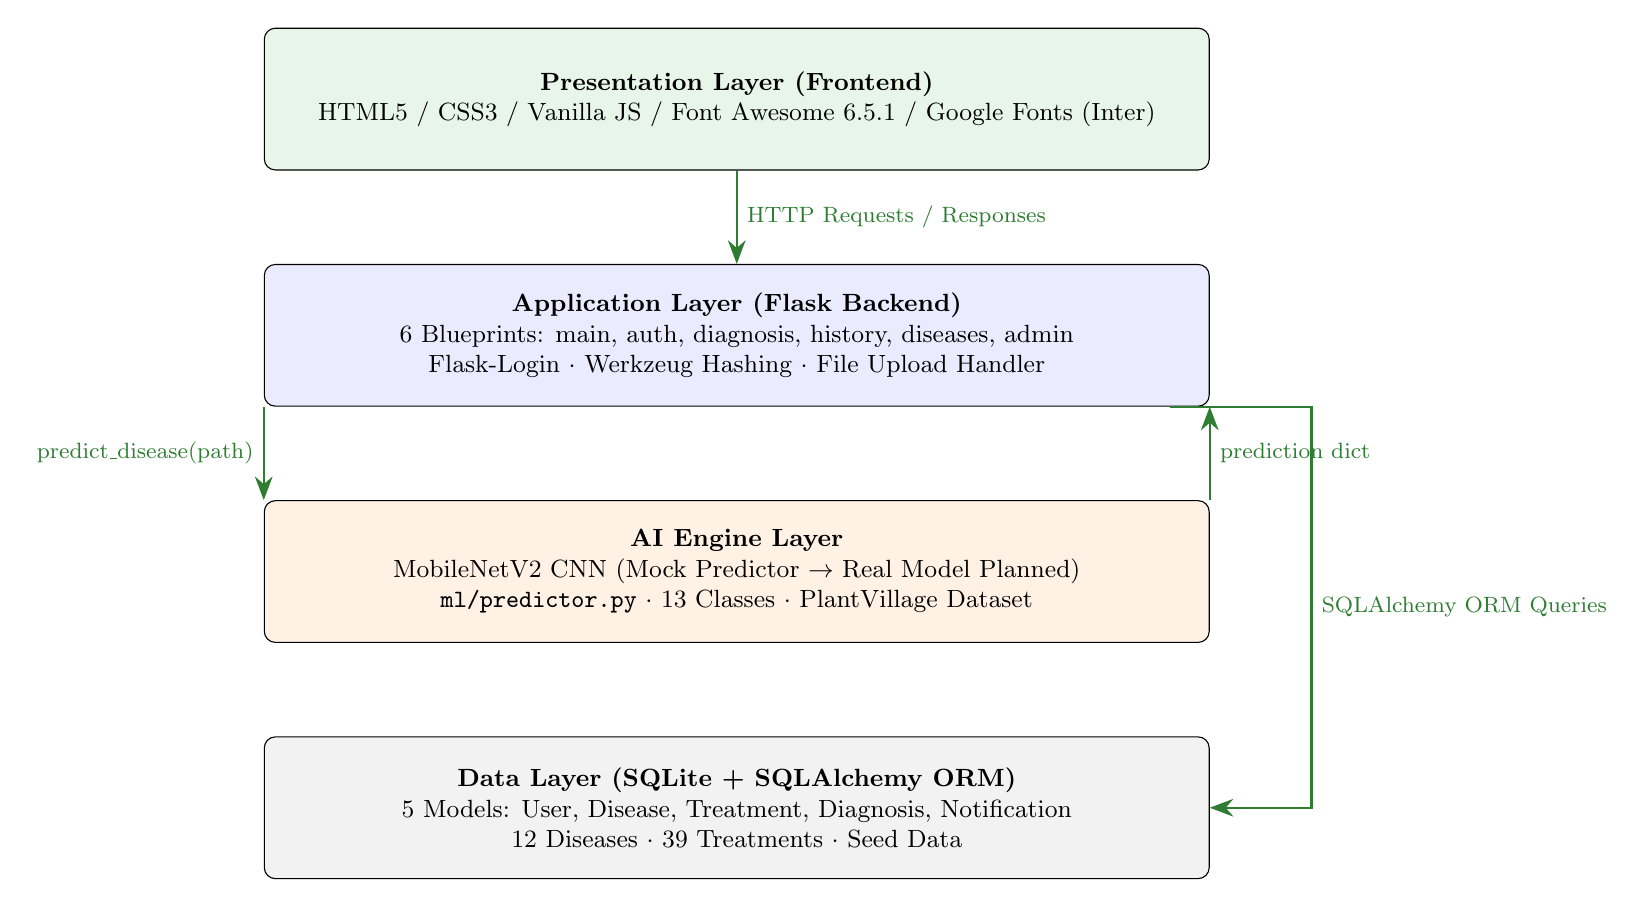
\begin{tikzpicture}[
    layer/.style={draw, rounded corners, minimum width=12cm,
                  minimum height=1.8cm, align=center, font=\small},
    arrow/.style={-{Stealth[length=3mm]}, thick, color=cropgreen},
    label/.style={font=\footnotesize\color{medgray}}
]
% --- layers ---
\node[layer, fill=lightgreen]               (fe) at (0,0)
  {\textbf{Presentation Layer (Frontend)}\\
   HTML5 / CSS3 / Vanilla JS / Font Awesome 6.5.1 / Google Fonts (Inter)};

\node[layer, fill=blue!8]                   (be) at (0,-3)
  {\textbf{Application Layer (Flask Backend)}\\
   6 Blueprints: main, auth, diagnosis, history, diseases, admin\\
   Flask-Login $\cdot$ Werkzeug Hashing $\cdot$ File Upload Handler};

\node[layer, fill=orange!10]                (ai) at (0,-6)
  {\textbf{AI Engine Layer}\\
   MobileNetV2 CNN (Mock Predictor $\rightarrow$ Real Model Planned)\\
   \texttt{ml/predictor.py} $\cdot$ 13 Classes $\cdot$ PlantVillage Dataset};

\node[layer, fill=gray!10]                  (db) at (0,-9)
  {\textbf{Data Layer (SQLite + SQLAlchemy ORM)}\\
   5 Models: User, Disease, Treatment, Diagnosis, Notification\\
   12 Diseases $\cdot$ 39 Treatments $\cdot$ Seed Data};

% --- arrows ---
\draw[arrow] (fe.south) -- node[right, label]{HTTP Requests / Responses} (be.north);
\draw[arrow] (be.south west) -- node[left, label]{predict\_disease(path)} (ai.north west);
\draw[arrow] (ai.north east) -- node[right, label]{prediction dict} (be.south east);
\draw[arrow] ([xshift=5.5cm]be.south) -- ++(1.8,0) |- node[near start, right, label]{SQLAlchemy ORM Queries} (db.east);

\end{tikzpicture}
\caption{CropGuard System Architecture (Four-Layer Design)}
\label{fig:arch}
\end{figure}

% ── User Interface and Hardware/Software Interfaces ──────
\subsection{User Interface}

The user interface is mobile-first with a responsive sidebar on larger screens. There are several UI design choices to note:

\begin{itemize}[leftmargin=2em]
  \item Homepage: Includes a hero section, feature grid (6 features), "how it works" steps, and call-to-action buttons. It is accessible without login.
  \item Dashboard: Displays scan metrics (number of scans, diseases detected, healthy results), recent scan results, unread notifications, and quick-action buttons.
  \item Diagnosis page: Provides a drag-and-drop upload area, camera capture button, crop type selector, and a loading spinner during disease prediction.
  \item Result page: Shows disease name in English and Bangla, a color-coded confidence bar, severity badge, image preview, and treatment tabs (chemical, organic, cultural).
  \item Admin page: Contains statistics cards, a user table, a disease management form, and a notification system with role-based targeting.
\end{itemize}

\subsection{Hardware Interface}

CropGuard does not rely on specialized hardware. The only hardware dependency is the user's camera, accessed through the HTML5 \texttt{capture="environment"} attribute on mobile devices. On desktop systems, a standard file selector is used instead. The backend can run on any machine with Python 3.10+ and at least 2\,GB of RAM.

\subsection{Software Interface}

\begin{itemize}[leftmargin=2em]
  \item AI integration: The Flask backend calls \texttt{predict\_disease(image\_path)} from \texttt{ml/predictor.py}. This function returns a dictionary containing the disease name, confidence score, severity, and top predictions. It can later be replaced with a TensorFlow model by modifying only this file.
  
  \item Database: SQLAlchemy ORM is used for all database operations. The system includes 5 models that handle CRUD functionality. The database is automatically created on first run and seeded using \texttt{seed\_data.py}.
  
  \item File storage: Uploaded images are stored in the \texttt{uploads/} directory using UUID-based filenames and are served through a dedicated Flask route.
\end{itemize}

\subsection{Survey (5 Farmer Respondents)}

\begin{itemize}[nosep]
    \item \textbf{Locations:} Ukhiya, Bancharumpur, Comilla, rural Dhaka.
    \item \textbf{Crops:} Boro Rice, Aman Rice, Potato, Tomato, Mango.
    \item \textbf{Key Findings:} 80\% experience frequent crop disease; 60\% rely on personal experience for identification; 80\% own smartphones; 20\% use farming apps.
    \item \textbf{Critical Insight (``Trust Gap''):} Farmers trust local pesticide shopkeepers more than technology. CropGuard must include human expert contact to bridge this gap.
\end{itemize}

\subsection{Document Analysis (15 Academic Papers)}

Papers analyzed across four themes:
\begin{enumerate}[nosep]
    \item \textbf{AI \& Deep Learning} (8 papers) --- Mohanty, Ferentinos, Sladojevic, Barbedo, Ramcharan, Too, Brahimi, Lu.
    \item \textbf{Mobile Deployment} (2 papers) --- Johannes, Arsenovic.
    \item \textbf{Crop Loss \& Food Security} (2 papers) --- Savary, Oerke.
    \item \textbf{Digital Agriculture} (3 papers) --- Deichmann, Qiang, Hughes \& Salath\'{e}.
\end{enumerate}



\section{Elicitation Results}
%==========================================================

Two approaches were used: \textbf{Surveys} (5 farmer respondents via Google Forms) and \textbf{Document Analysis} (15 academic papers).

\subsection{Survey Results}

\textbf{Demographics:} 5 respondents from Ukhiya, Bancharumpur, Comilla, and rural Dhaka. Age 26--50, 10+ years farming experience, farm size 0.5--2.0 acres. Primary crops: Boro Rice, Aman Rice, Potato, Tomato, Mango.

\begin{table}[h!]
\centering
\small
\begin{tabularx}{\textwidth}{|l|c|X|}
\hline
\rowcolor{lightgreen}
\textbf{Finding} & \textbf{Value} & \textbf{Insight} \\
\hline
Disease frequency (Very Frequent + Occasional) & 80\% & Crop disease is a widespread, recurring problem. \\
\hline
Common diseases & -- & Rice Blast, Leaf Blight, Pest Infestations, Root Rot. \\
\hline
Identification method & 60\% & Rely on personal experience; 20\% consult pesticide dealers. \\
\hline
Time to identify & 1--3 days & Significant delay causing further crop damage. \\
\hline
Smartphone ownership & 80\% & Hardware accessibility is not a barrier. \\
\hline
Internet access & 80\% & Connectivity available in target regions. \\
\hline
Farming app usage & 20\% & Gap in market  farmers use Facebook/YouTube, not farming apps. \\
\hline
Willingness to pay & Moderate & Prefer freemium or low-cost per-use model. \\
\hline
\end{tabularx}
\caption{Key survey findings}
\end{table}

\textbf{Key Insight --- ``Trust Gap'':} Farmers trust local pesticide shopkeepers more than any other source. CropGuard must act as a reliable, unbiased ``Digital Expert'' that delivers results in seconds (vs.\ 1--3 days currently).

\subsection{Document Analysis Results}

Fifteen academic papers were analyzed across four themes. Key findings are summarized below; full citations appear in the References section.

\subsubsection*{(a) AI \& Deep Learning for Plant Disease Detection (8 papers)}

\begin{itemize}[leftmargin=*, nosep]
    \item \textbf{Mohanty et al.\ (2016):} CNNs achieved 99.35\% accuracy on 54,306 leaf images  validates AI-based diagnosis feasibility.
    \item \textbf{Ferentinos (2018):} Transfer learning with VGG/ResNet reached 99.48\% on 87,848 images  confirms high accuracy is reproducible.
    \item \textbf{Sladojevic et al.\ (2016):} CaffeNet-based model achieved 96.3\% on 13 disease classes  demonstrates real-world applicability.
    \item \textbf{Barbedo (2019):} Individual lesion-level detection improves early-stage diagnosis  supports fine-grained analysis.
    \item \textbf{Ramcharan et al.\ (2017):} Deep learning on cassava diseases in field conditions  proves effectiveness beyond lab settings.
    \item \textbf{Too et al.\ (2019):} DenseNet outperformed VGG16 and InceptionV4  guides model architecture selection for CropGuard.
    \item \textbf{Brahimi et al.\ (2017):} Visualization of learned features for tomato diseases supports interpretable AI results.
    \item \textbf{Lu et al.\ (2017):} CNN identification of 10 rice diseases with 95.48\% accuracy  directly relevant to Bangladesh rice farming.
\end{itemize}

\subsubsection*{(b) Mobile \& Practical Deployment (2 papers)}

\begin{itemize}[leftmargin=*, nosep]
    \item \textbf{Johannes et al.\ (2017):} Mobile-captured images achieve comparable accuracy to lab images validates smartphone-based diagnosis.
    \item \textbf{Arsenovic et al.\ (2019):} Addressed real-world challenges (lighting, background noise) in plant disease detection informs CropGuard's image preprocessing.
\end{itemize}

\subsubsection*{(c) Crop Loss \& Food Security (2 papers)}

\begin{itemize}[leftmargin=*, nosep]
    \item \textbf{Savary et al.\ (2019):} Plant diseases cause 10--40\% annual crop losses globally (\$220B)  establishes the problem's scale.
    \item \textbf{Oerke (2006):} Without crop protection, potential losses reach 50--80\% for major staples  underscores urgency of early detection.
\end{itemize}

\subsubsection*{(d) Digital Agriculture \& Datasets (3 papers)}

\begin{itemize}[leftmargin=*, nosep]
    \item \textbf{Deichmann et al.\ (2016):} Mobile penetration exceeds 80\% in rural developing areas confirms web platform accessibility.
    \item \textbf{Qiang et al.\ (2011):} Mobile apps reduce agricultural information asymmetry by 60\%  supports CropGuard's advisory model.
    \item \textbf{Hughes \& Salath\'{e} (2015):} PlantVillage open dataset with 54,000+ images  primary training data source for CropGuard's CNN.
\end{itemize}

%==========================================================
\section{Latest Features from Fieldwork}
%==========================================================

Based on farmer survey responses, the following 10 features were identified as most needed. Each feature is linked to specific survey findings and user pain points observed during the elicitation process.

\begin{longtable}{|c|L{3cm}|L{10.5cm}|}
\caption{Features derived from fieldwork with detailed user needs} \\
\hline
\rowcolor{lightgreen}
\textbf{\#} & \textbf{Feature} & \textbf{User Need (from Survey)} \\
\hline
\endfirsthead
\hline
\rowcolor{lightgreen}
\textbf{\#} & \textbf{Feature} & \textbf{User Need (from Survey)} \\
\hline
\endhead

F1 & Camera-Based Leaf Scanning & 80\% of respondents prefer camera over typing. Farmers want to point their phone at a diseased leaf and receive instant results without navigating complex menus critical for low-literacy users working in the field. \\
\hline
F2 & Instant AI Diagnosis & 80\% ranked speed as the top priority. Currently, farmers wait 1-3 days visiting pesticide dealers or extension offices. AI diagnosis in under 5 seconds prevents further crop damage during the identification delay. \\
\hline
F3 & Treatment in Bangla & 60\% of farmers struggle with English-only agricultural advice. Bangla-language descriptions using locally familiar terms (e.g., local pesticide brand names) significantly improve comprehension and treatment adoption rates. \\
\hline
F4 & Organic Treatment Options & 40\% actively seek organic or cultural alternatives to chemical pesticides due to health concerns, rising input costs, and growing awareness of environmental impact. They want at least one non-chemical option per disease. \\
\hline
F5 & Expert Contact (Call/WhatsApp) & Farmers trust human experts more than technology alone. One-tap Call and WhatsApp buttons let farmers verify AI results with a real agricultural officer directly addressing the ``trust gap'' revealed in survey responses. \\
\hline
F6 & Diagnosis History & Farmers want to track which diseases appeared on their farm and when. Seasonal history enables pattern recognition (e.g., recurring Blast every Aman season) and informs preventive measures for future planting cycles. \\
\hline
F7 & Disease Library & Farmers want to browse diseases proactively before symptoms appear. A visual reference library with photos, symptom descriptions, and treatment options enables self-education and early preparedness. \\
\hline
F8 & Offline-Friendly Design & Rural areas in Ukhiya and Bancharumpur experience intermittent 2G/3G connectivity. Pages must be lightweight ($<$500KB) to load on slow networks and remain usable during brief connectivity windows. \\
\hline
F9 & Emergency Helplines & During severe outbreaks (e.g., rice blast epidemic), farmers need immediate government support. Quick-dial access to the DAE helpline (16123) and Krishi Call Center reduces emergency response time from hours to seconds. \\
\hline
F10 & Notification Alerts & Regional disease outbreaks spread rapidly across adjacent farms. Timely push notifications warn nearby farmers to take preventive action (e.g., apply fungicide) before infection reaches their fields. \\
\hline
\end{longtable}

\textbf{Key Observations:} Features F1, F2, and F5 address the three most critical pain points: (1)~ease of input for non-technical users, (2)~speed of diagnosis vs.\ the current 1--3 day delay, and (3)~building trust through human expert validation. Features F3 and F4 reflect Bangladesh-specific needs not addressed by existing global plant disease apps. Features F8-F10 address infrastructure and emergency preparedness challenges unique to rural farming communities.

%==========================================================
\section{Feature Comparison: Literature vs.\ Fieldwork}
%==========================================================

\begin{table}[h!]
\centering
\small
\begin{tabularx}{\textwidth}{|L{3.5cm}|C{1.8cm}|C{1.8cm}|X|}
\hline
\rowcolor{lightgreen}
\textbf{Feature} & \textbf{Literature} & \textbf{Fieldwork} & \textbf{Analysis} \\
\hline
AI Disease Detection & \checkmark & \checkmark & Core feature validated by both sources. \\
\hline
Image Upload (Camera) & \checkmark & \checkmark & Fieldwork confirmed camera-first interaction preference. \\
\hline
Treatment Recommendations & \checkmark & \checkmark & Fieldwork added demand for organic \& cultural methods. \\
\hline
Diagnosis History & \checkmark & \checkmark & Both support tracking past diagnoses. \\
\hline
Disease Library & \checkmark & \checkmark & Both support a browseable knowledge base. \\
\hline
Multi-Crop Support & \checkmark & \checkmark & Fieldwork confirmed Rice, Potato, Tomato, Mango priority. \\
\hline
User Authentication & \checkmark & \checkmark & Standard requirement from both. \\
\hline
Admin Dashboard & \checkmark & -- & System design need; not farmer-facing. \\
\hline
Bangla Language Support & -- & \checkmark & \textbf{New.} Strongly demanded by farmers. \\
\hline
Expert Contact & -- & \checkmark & \textbf{New.} Addresses farmer ``trust gap''. \\
\hline
Notification Alerts & -- & \checkmark & \textbf{New.} Regional outbreak warnings. \\
\hline
Emergency Helplines & -- & \checkmark & \textbf{New.} Government agriculture lines (16123). \\
\hline
Offline-Friendly Design & -- & \checkmark & \textbf{New.} Critical for rural connectivity. \\
\hline
\end{tabularx}
\caption{Literature vs.\ Fieldwork comparison}
\end{table}

\textbf{Key Takeaway:} Fieldwork added 5 new features not found in literature, demonstrating the value of direct stakeholder engagement.



% ══════════════════════════════════════════════════════════
%  3. SPECIFIC REQUIREMENTS
% ══════════════════════════════════════════════════════════
\section{Specific Requirements}

This section provides an overview of the functionality of CropGuard, by component. We start with user stories (to demonstrate why) and then go on to the functional requirements in the Actor-Trigger-Criteria format.

% ── Use Case Diagram ─────────────────────────────────────
\subsection{Use Case Diagram}

Figure~\ref{fig:usecase} gives an overview of the interactions between the four types of users and the system.

\begin{figure}[H]
\centering
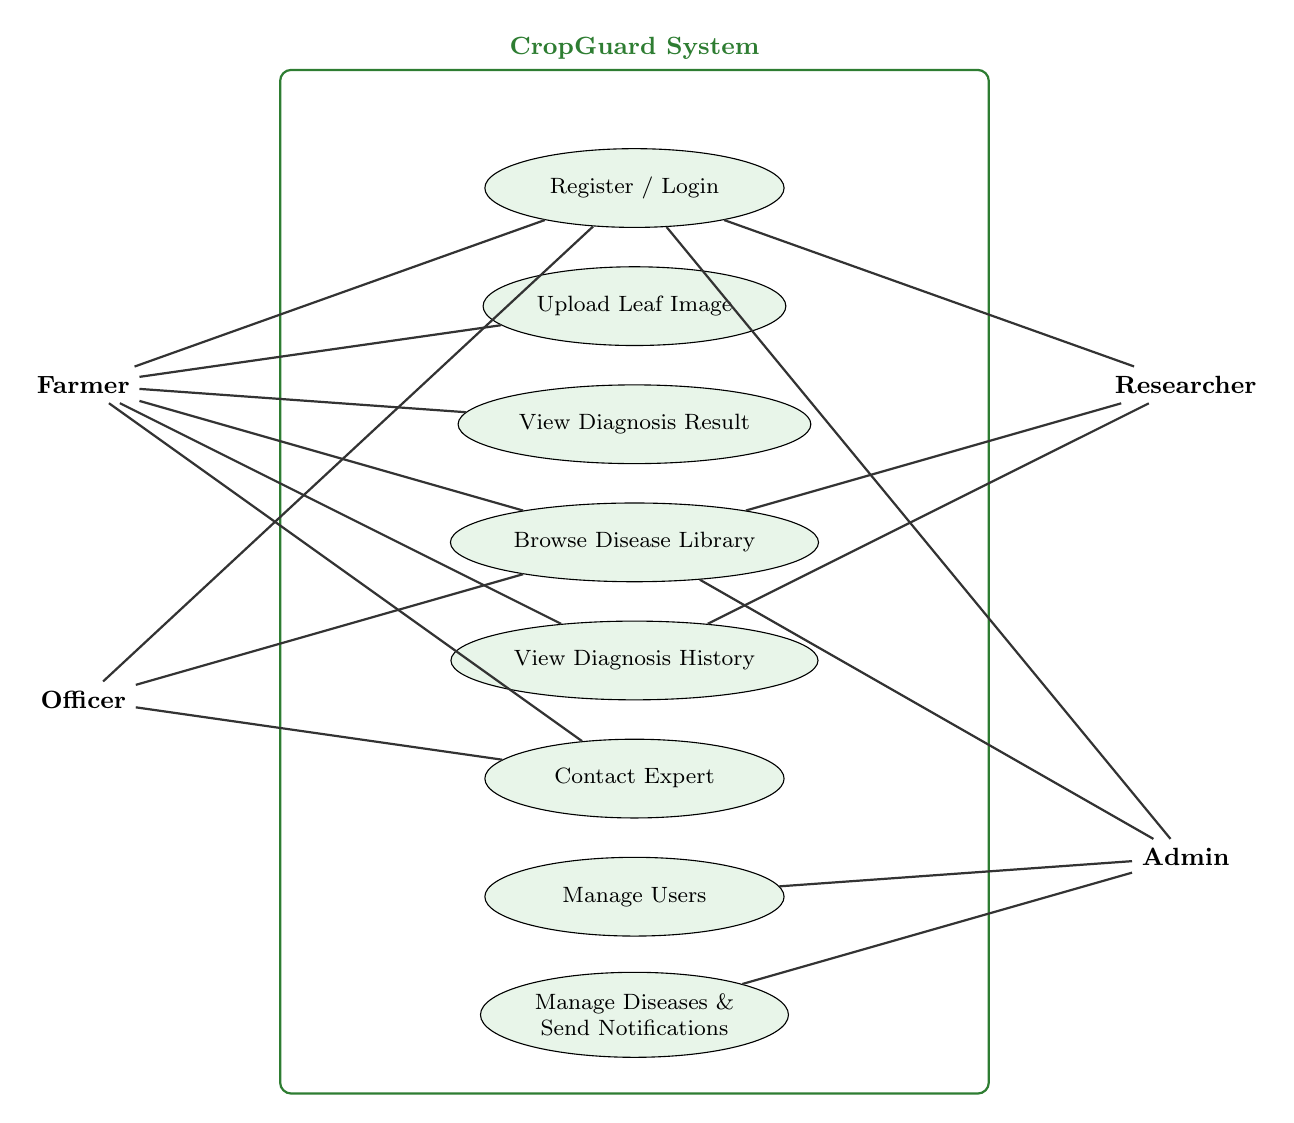
\begin{tikzpicture}[
    actor/.style={font=\small\bfseries},
    usecase/.style={draw, ellipse, minimum width=3.8cm, minimum height=1cm,
                    align=center, font=\footnotesize, fill=lightgreen},
    sysbox/.style={draw=cropgreen, thick, rounded corners, inner sep=12pt},
    conn/.style={-, thick, color=darkgray}
]

% --- system boundary ---
\node[sysbox, minimum width=9cm, minimum height=13cm, label={[font=\small\bfseries\color{cropgreen}]above:CropGuard System}] (sys) at (5.5,-5.5) {};

% --- use cases ---
\node[usecase] (uc1) at (5.5, -0.5) {Register / Login};
\node[usecase] (uc2) at (5.5, -2.0) {Upload Leaf Image};
\node[usecase] (uc3) at (5.5, -3.5) {View Diagnosis Result};
\node[usecase] (uc4) at (5.5, -5.0) {Browse Disease Library};
\node[usecase] (uc5) at (5.5, -6.5) {View Diagnosis History};
\node[usecase] (uc6) at (5.5, -8.0) {Contact Expert};
\node[usecase] (uc7) at (5.5, -9.5) {Manage Users};
\node[usecase] (uc8) at (5.5,-11.0) {Manage Diseases \&\\Send Notifications};

% --- actors (left: Farmer / Officer) ---
\node[actor] (farmer) at (-1.5, -3.0) {Farmer};
\node[actor] (officer) at (-1.5, -7.0) {Officer};

% --- actors (right: Researcher / Admin) ---
\node[actor] (researcher) at (12.5, -3.0) {Researcher};
\node[actor] (admin)      at (12.5, -9.0) {Admin};

% --- connections: farmer ---
\draw[conn] (farmer) -- (uc1);
\draw[conn] (farmer) -- (uc2);
\draw[conn] (farmer) -- (uc3);
\draw[conn] (farmer) -- (uc4);
\draw[conn] (farmer) -- (uc5);
\draw[conn] (farmer) -- (uc6);

% --- connections: officer ---
\draw[conn] (officer) -- (uc1);
\draw[conn] (officer) -- (uc4);
\draw[conn] (officer) -- (uc6);

% --- connections: researcher ---
\draw[conn] (researcher) -- (uc1);
\draw[conn] (researcher) -- (uc4);
\draw[conn] (researcher) -- (uc5);

% --- connections: admin ---
\draw[conn] (admin) -- (uc1);
\draw[conn] (admin) -- (uc7);
\draw[conn] (admin) -- (uc8);
\draw[conn] (admin) -- (uc4);

\end{tikzpicture}
\caption{Use Case Diagram CropGuard Actor Interactions}
\label{fig:usecase}
\end{figure}

% ── Sequence Diagram ─────────────────────────────────────
\subsection{Sequence Diagram --- Leaf Scan Flow}

Figure~\ref{fig:sequence} shows the entire process from image upload to result, including the interactions between the user, Flask backend, AI engine, and the database.

\begin{figure}[H]
\centering
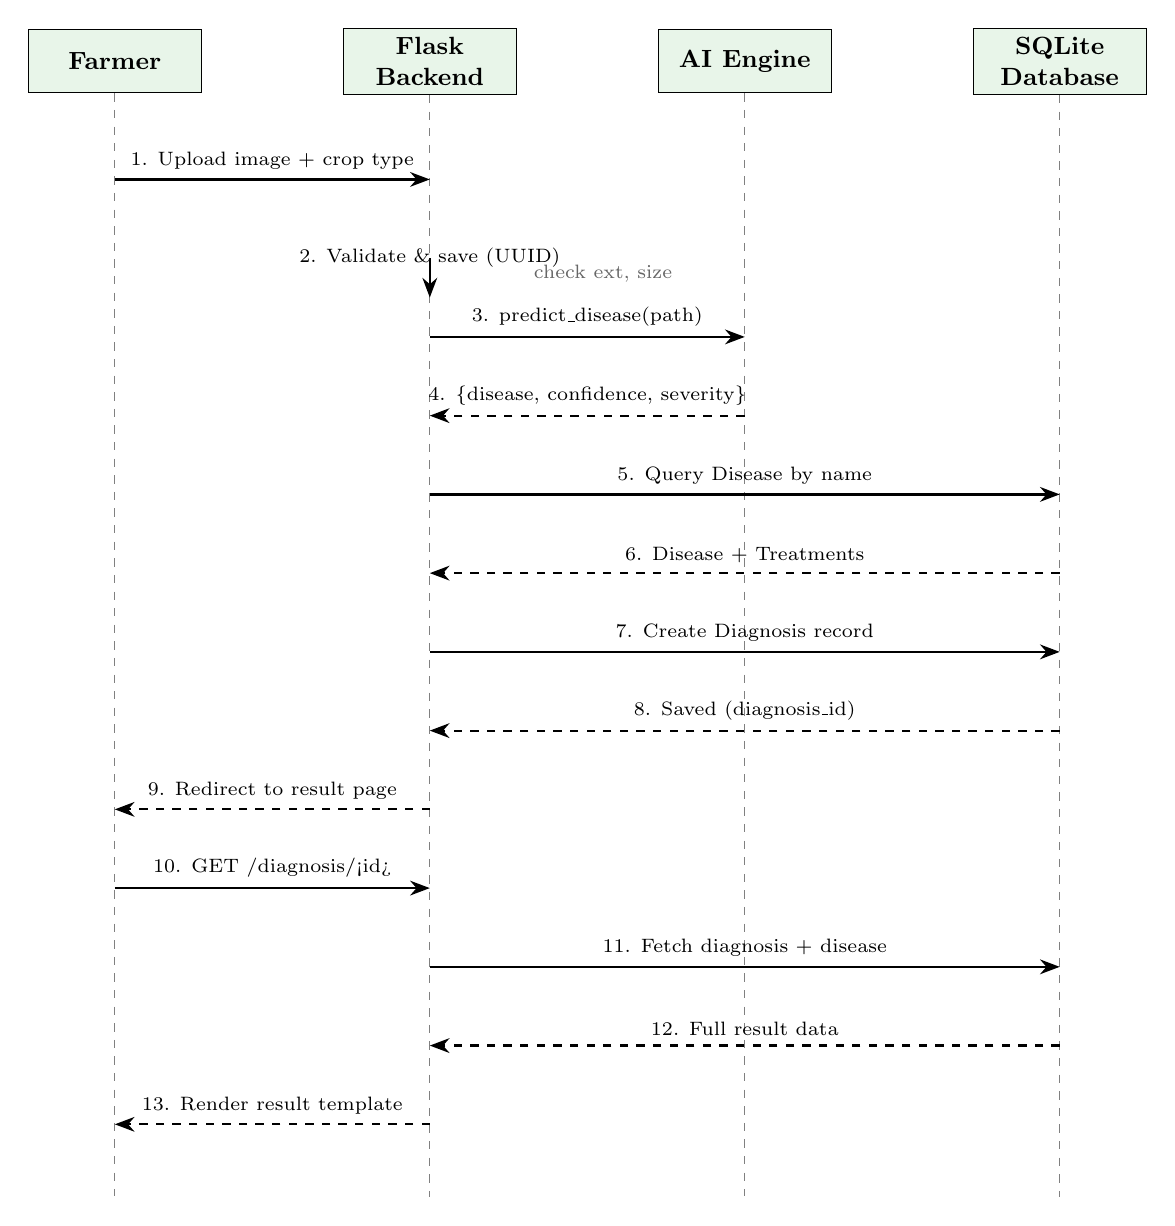
\begin{tikzpicture}[
    entity/.style={draw, rectangle, minimum width=2.2cm, minimum height=0.8cm,
                   fill=lightgreen, font=\small\bfseries, align=center},
    msg/.style={-{Stealth[length=2.5mm]}, thick},
    rmsg/.style={-{Stealth[length=2.5mm]}, thick, dashed},
    note/.style={font=\scriptsize, align=left, color=medgray}
]

% --- entities ---
\node[entity] (user) at (0,0)   {Farmer};
\node[entity] (flask) at (4,0)  {Flask\\Backend};
\node[entity] (ai) at (8,0)     {AI Engine};
\node[entity] (db) at (12,0)    {SQLite\\Database};

% --- lifelines ---
\draw[dashed, gray] (user.south)  -- ++(0,-14);
\draw[dashed, gray] (flask.south) -- ++(0,-14);
\draw[dashed, gray] (ai.south)    -- ++(0,-14);
\draw[dashed, gray] (db.south)    -- ++(0,-14);

% --- messages ---
\draw[msg] (0,-1.5) -- node[above, font=\scriptsize]{1. Upload image + crop type} (4,-1.5);

\draw[msg] (4,-2.5) -- node[above, font=\scriptsize]{2. Validate \& save (UUID)} (4,-3.0);
\node[note] at (6.2,-2.7) {check ext, size};

\draw[msg] (4,-3.5) -- node[above, font=\scriptsize]{3. predict\_disease(path)} (8,-3.5);

\draw[rmsg] (8,-4.5) -- node[above, font=\scriptsize]{4. \{disease, confidence, severity\}} (4,-4.5);

\draw[msg] (4,-5.5) -- node[above, font=\scriptsize]{5. Query Disease by name} (12,-5.5);

\draw[rmsg] (12,-6.5) -- node[above, font=\scriptsize]{6. Disease + Treatments} (4,-6.5);

\draw[msg] (4,-7.5) -- node[above, font=\scriptsize]{7. Create Diagnosis record} (12,-7.5);

\draw[rmsg] (12,-8.5) -- node[above, font=\scriptsize]{8. Saved (diagnosis\_id)} (4,-8.5);

\draw[rmsg] (4,-9.5) -- node[above, font=\scriptsize]{9. Redirect to result page} (0,-9.5);

\draw[msg] (0,-10.5) -- node[above, font=\scriptsize]{10. GET /diagnosis/<id>} (4,-10.5);

\draw[msg] (4,-11.5) -- node[above, font=\scriptsize]{11. Fetch diagnosis + disease} (12,-11.5);

\draw[rmsg] (12,-12.5) -- node[above, font=\scriptsize]{12. Full result data} (4,-12.5);

\draw[rmsg] (4,-13.5) -- node[above, font=\scriptsize]{13. Render result template} (0,-13.5);

\end{tikzpicture}
\caption{Sequence Diagram Leaf Scan from Upload to Result Display}
\label{fig:sequence}
\end{figure}


% ── Component 1 ──────────────────────────────────────────
\subsection{Component 1: Farmer Registration and Authentication}

\subsubsection*{User Stories}

\begin{enumerate}[leftmargin=2em]
  \item A farmer want to register with their name, email, phone number and address - so that the diagnosis history is stored and they can view it later.
  \item And they want to easily login and be remembered (the ``remember me'' option) so that they don't have to put the password every time.
  \item And if they try to register with a duplicate email, it should not allow them to do so, so they know if they have an account or not.
\end{enumerate}

\subsubsection*{Functional Requirements}

\frbox{FR-01: User Registration}
{Smallholder farmers, extension officers or researchers}
{They click the ``Register'' button and fill out the form for name, email, phone, password, role and location.}
{It then validates the form, ensuring no-one has the same email address, hash the password using Werkzeug PBKDF2-SHA256, insert a new User record and automatically logs them in, then redirect to the dashboard.}
{%
\begin{itemize}[leftmargin=1.5em]
  \item all mandatory fields (name, email, phone, password, role) must be entered, and if any are missing the validation error message appears inline;
  \item if the email is already in the system a specific error message saying ``Email already registered'' needs to be displayed;
  \item the password must be stored as a salted hash, never as plaintext;
  \item the user is automatically logged in and redirected to the dashboard after successful registration.
\end{itemize}
}

\frbox{FR-02: User Login}
{Registered users}
{Users visit \texttt{/login}, enter email and password.}
{It verifies that the email exists, and the password hash using Werkzeug's \texttt{check\_password\_hash}. If successful, a Flask-Login session is established (with optional remember me). On error, it displays a generic error.}
{%
\begin{itemize}[leftmargin=1.5em]
  \item correct credentials redirect to dashboard;
  \item incorrect credentials display ``Invalid email or password'' (it can't be known if the email or the password is incorrect);
  \item check box for ``Remember Me'' when checked, makes the session persistent over browser restart.
\end{itemize}
}

\frbox{FR-03: User Logout}
{Authenticated user}
{The user clicks on ``Logout'' in the sidebar.}
{The session is cleared, both Flask-Login's session and the session cookie, and redirects to the login page.}
{%
\begin{itemize}[leftmargin=1.5em]
  \item after the user logout, attempt to access any page must redirect to \texttt{/login};
  \item the session cookie must be invalidated on the server side.
\end{itemize}
}

\frbox{FR-04: Role-Based Access Control}
{All users}
{A user could try to reach an url that requires a role (such as \texttt{/admin/}).}
{It will check the user role. To access admin routes, you need role=admin. If not they receive an HTTP 403 Forbidden message.}
{%
\begin{itemize}[leftmargin=1.5em]
  \item users not logged in get redirected to the login screen;
  \item those logged in but not admin get a 403 when visiting \texttt{/admin/*} routes;
  \item admins can do anything.
\end{itemize}
}

% ── Component 2 ──────────────────────────────────────────
\subsection{Component 2: Disease Diagnosis and AI}
\subsubsection*{User Stories}

\begin{itemize}[leftmargin=2em]
  \item The farmer want to hold up their mobile phone to a diseased leaf and get an answer - without needing to find out how to do this.
  \item They want to see the name of the disease in Bangla and English, as they may not know the English names.
  \item And they want to know how sure it is, so they know if they can rely on it or need to seek another opinion.
  \item And they want to be able to indicate whether the diagnosis was useful or not, so that the system can learn how accurate it is getting.
\end{itemize}

\subsubsection*{Functional Requirements}

\frbox{FR-05: Uploading and taking photos}
{Smallholder farmer}
{They visit \texttt{/diagnosis} and select an image of a leaf one of the three ways: file selection, drag and drop into the upload area, or directly from the camera (HTML5 \texttt{capture="environment"}).}
{The JavaScript on the client side checks the file format and size, displays a thumbnail and activates the Diagnose button only if the user has also selected a crop type from the dropdown list (Rice, Potato, Tomato, Mango, Other).}
{%
\begin{itemize}[leftmargin=1.5em]
  \item only JPEG, PNG, WebP files are accepted (in which case it should say ``Other formats are not supported'') - other formats should be rejected with a message;
  \item maximum file size is 10 MB, larger files must be blocked before upload;
  \item immediately after the image is selected, a thumbnail appears;
  \item the Diagnose button is disabled until both image and crop type are selected.
\end{itemize}
}

\frbox{FR-06: AI Disease Diagnosis}
{Smallholder farmer}
{Farmer clicks ``Diagnose'' once image and crop type are chosen.}
{The server stores the image in \texttt{uploads/} directory with a filename based on a UUID and passes the path to \texttt{ml/predictor.py}'s \texttt{predict\_disease(image\_path)}. The dictionary returned contains disease name, confidence, severity, and top\_n predictions. It does a lookup in the Disease table to find the disease, creates a Diagnosis record connecting the user, image, disease, crop, and confidence, and finally redirects to the result page.}
{%
\begin{itemize}[leftmargin=1.5em]
  \item the result page should display the name of the disease in English and Bangla (from \texttt{name\_bn});
  \item confidence score (0-100\%) represented by a bar (green if 80\% or more, yellow 50-79\%, red less than 50\%);
  \item severity appears as a badge: Low, Medium, High, or Critical;
  \item the uploaded leaf image is visible on the result page;
  \item at least one chemical and one organic treatment must be displayed (pulled from the Treatment table).
\end{itemize}
}

\frbox{FR-07: Treatment Display}
{Smallholder farmer}
{Diagnosis results in a page with treatments from the Treatment table, filtered by the disease.}
{They are tabbed as Chemical, Organic and Cultural. Chemical treatments include name, dose, route, and precautions.}
{%
\begin{itemize}[leftmargin=1.5em]
  \item there are three tabs;
  \item each treatment shows at least the name and description;
  \item chemical treatments also show the dosage and precautions (if applicable).
\end{itemize}
}

\frbox{FR-08: Diagnosis Feedback}
{Smallholder farmer}
{The farmer can click on the result page a button ``Effective'' (thumbs up) or ``Not Effective'' (thumbs down) and optionally provide comments.}
{The Diagnosis record's feedback and feedback\_notes are updated. Feedback can be given only by the creator of the diagnosis.}
{%
\begin{itemize}[leftmargin=1.5em]
  \item two feedback buttons (thumbs up and down);
  \item an optional text notes field for additional comments;
  \item feedback is stored on the existing Diagnosis record, not in a separate feedback table;
  \item only the creator of the diagnosis can submit feedback.
\end{itemize}
}

\frbox{FR-09: Diagnosis History}
{Smallholder farmer / researcher}
{Farmer (or researcher) visits \texttt{/history}.}
{It takes the Diagnosis records associated with the user, ordered by date (newest first) and presents them in a list.}
{%
\begin{itemize}[leftmargin=1.5em]
  \item it lists each diagnosis with thumbnail image, name, crop, date, confidence level and whether the diagnosis has been checked;
  \item shows the most recent diagnosis first;
  \item lists only diagnoses made by the user.
\end{itemize}
}


% ── Component 3 ──────────────────────────────────────────
\subsection{Component 3: Disease Library and Treatment Advisory}

\subsubsection*{User Stories}

\begin{itemize}[leftmargin=2em]
  \item The farmer would like to browse a list of common crop diseases, to find out what to look out for, so their crops don't fall ill.
  \item They want to search by disease name and filter by crop type, to find the info they need.
  \item The researcher wants to see the symptoms, causes and all treatment methods for the disease.
\end{itemize}

\subsubsection*{Functional Requirements}

\frbox{FR-10: Browse Diseases}
{All users}
{The Disease Library page (\texttt{/diseases}) can be accessed by anyone.}
{It loads all diseases from the database and displays them in a grid. The card shows the English name, Bangla name, affected crop, severity badge and brief description.}
{%
\begin{enumerate}[leftmargin=1.5em, topsep=0pt]
  \item We should see all 12 seed diseases - Rice Blast, Rice Brown Spot, Rice Leaf Blight, Rice Sheath Blight, Rice Tungro, Potato Late Blight, Potato Early Blight, Tomato Early Blight, Tomato Late Blight, Tomato Leaf Curl, Mango Anthracnose, Mango Powdery Mildew.
  \item English and Bangla names are shown in the cards.
  \item The card takes us to the detail page for the disease.
\end{enumerate}
}

\frbox{FR-11: Filter and Search for Diseases}
{All users}
{A user can enter search keywords, and select a crop from the filter menu.}
{It matches on the server-side, partial matching on name, Bangla name and description. The crop filter narrows down to that crop; crops are All, Rice, Potato, Tomato, Mango.}
{%
\begin{enumerate}[leftmargin=1.5em, topsep=0pt]
  \item search does partial matches (so ``Blast'' gives ``Rice Blast'').
  \item the crop filter gives only those of the specified crop.
  \item search and crop filter together gives only diseases that match both search and crop.
\end{enumerate}
}

\frbox{FR-12: View Disease Page}
{All users}
{Clicking a disease card takes you to \texttt{/diseases/<id>}.}
{The page displays all details of the disease: description, symptoms, causes, and treatments linked to the disease, separated by treatment type.}
{%
\begin{enumerate}[leftmargin=1.5em, topsep=0pt]
  \item full description, symptoms and causes are shown.
  \item treatments are grouped into Chemical, Organic and Cultural.
  \item the name, description and (for chemical treatments) dosage and precautions are displayed.
\end{enumerate}
}

% ── Component 4 ──────────────────────────────────────────
\subsection{Component 4: Contact an Expert and Emergency Info}

\subsubsection*{User Stories}

\begin{itemize}[leftmargin=2em]
  \item I'm a farmer and I want to reach out to an ag expert (by phone, email or WhatsApp) if I'm unsure about a diagnosis.
  \item And I wanna see the emergency phone numbers straight away, in case I need to call during an outbreak.
\end{itemize}

\subsubsection*{Functional Requirements}

\frbox{FR-13: Contact Expert}
{Smallholder farmer}
{They go to the Contact Expert page.}
{It shows a list of all extension officers, with their name, phone and email. Next, there are buttons that allow you to call (tel:), send WhatsApp (wa.me/), or send email (mailto:) to each officer.}
{%
\begin{enumerate}[leftmargin=1.5em, topsep=0pt]
  \item all extension officers (with role = officer) must be listed.
  \item each officer must have Call, WhatsApp, and Email buttons.
  \item buttons must use the correct URI schemes - tel:, https://wa.me/, mailto:.
\end{enumerate}
}

\frbox{FR-14: Emergency Helplines}
{All users}
{When they open up the Contact Expert page, they see DAE Helpline (16123) and Krishi Call Center (3331) really big at the top.}
{The system displays emergency numbers prominently.}
{%
\begin{enumerate}[leftmargin=1.5em, topsep=0pt]
  \item the 2 helpline numbers must be above the fold.
  \item they must be clickable (using tel: links) on mobile.
\end{enumerate}
}

% ── Component 5 ──────────────────────────────────────────
\subsection{Component 5: Admin Panel}

\subsubsection*{User Stories}

\begin{itemize}[leftmargin=2em]
  \item I want, as an admin, a snapshot of overall status - users, diagnoses, diseases.
  \item I need to add new diseases when an outbreak of an unregistered disease occurs.
  \item I want to disable accounts of users abusing the system.
  \item I want to notify all farmers or all officers of an outbreak.
\end{itemize}

\subsubsection*{Functional Requirements}

\frbox{FR-15: Admin Dashboard}
{System administrator}
{The system administrator logs in and clicks on \texttt{/admin/}.}
{The dashboard displays statistics: number of users, farmers, officers, diagnoses, and diseases. Below the stats, there are tables of the top 10 diagnoses and top 10 user registrations.}
{%
\begin{enumerate}[leftmargin=1.5em, topsep=0pt]
  \item only users with role = admin can access it.
  \item the five stats (users, farmers, officers, diagnoses, diseases) must be shown.
  \item recent diagnoses and registrations must be ordered by date, descending.
\end{enumerate}
}

\frbox{FR-16: User Management}
{System administrator}
{Admin navigates to \texttt{/admin/users}.}
{It displays all users with their name, email, role, location, status (active or not), and date of registration. The admin can change user’s status with a click of a button.}
{%
\begin{enumerate}[leftmargin=1.5em, topsep=0pt]
  \item all users show up with full details.
  \item admin can make any user's is_active status true or false.
  \item admin cannot make his/her own account inactive.
  \item status is updated immediately.
\end{enumerate}
}

\frbox{FR-17: Disease Management}
{System administrator}
{Admin visits \texttt{/admin/diseases} and enters information into the ``Add Disease'' form.}
{A new Disease is created with name, Bangla name (name\_bn), crop, severity, description, symptoms, and causes. The new disease then shows up in the Disease Library.}
{%
\begin{enumerate}[leftmargin=1.5em, topsep=0pt]
  \item fields accepted in form are: name, Bangla name, crop, severity, description, symptoms, causes.
  \item the new disease will appear without server restart.
  \item (Note: updating and removing diseases is not supported yet.)
\end{enumerate}
}

\frbox{FR-18: Notification System}
{System administrator}
{Admin writes a notification (title, message, target).}
{For each user in the target (All, Farmers, Officers), the system generates a Notification record. The notifications are displayed on user dashboards.}
{%
\begin{enumerate}[leftmargin=1.5em, topsep=0pt]
  \item target must be All, Farmers, Officers.
  \item a Notification record is created for each user in the target.
  \item notifications appear on dashboards with a read/unread flag.
  \item users can set them as read.
\end{enumerate}
}


% ══════════════════════════════════════════════════════════
%  3.X  MAA JUSTIFICATION
% ══════════════════════════════════════════════════════════
\subsection{Minimum Acceptable Accuracy (MAA) Justification}
\label{sec:maa}

CropGuard's AI engine aims for a target MAA of 85\% on the PlantVillage validation set for the 12 target diseases. This is not an arbitrary number, but reflects the balance of three factors:

\begin{enumerate}[leftmargin=2em]
  \item Current baseline. Farmers now seem to only achieve an 85\% accuracy in diagnosing diseases purely by experience, according to our survey. So 85% is a 25% increase. That's a significant boost over the way things are now.

  \item Literature benchmarks. The PlantVillage papers report lab accuracy of 95-99\% (Mohanty et al., 2016; Ferentinos, 2018). That's a good thing, but it's also a little misleading. Ramcharan et al. (2017) demonstrated models that work well on clean, lab-condition images can fall 10-15\% when applied to real images from the field (different lighting, angles, sometimes multiple diseases per leaf).

  \item Global crop loss context. Savary et al. (2019) report 10-40\% of crops are lost globally to pests and diseases. If CropGuard can catch even some of these cases sooner, that could make a big economic difference to a smallholder farmer. But 95\% accuracy in the field is not achievable on the current training approach. And if we put in a system that isn't hitting the right target, then farmers won't have confidence - and that's the last thing we want to do.
\end{enumerate}

So 85\% is achievable in the field. If later field studies reveal it may be too high (or perhaps too low), we will be able to alter the threshold based on the feedback data we get from the "Effective / Not Effective" feature (FR-08).

\section{S.M.A.R.T. Justification of Selected Features}
%==========================================================

Each selected feature is justified using the \textbf{S.M.A.R.T.} framework (Specific, Measurable, Achievable, Relevant, Time-bound).

\renewcommand{\arraystretch}{1.3}

\subsection{AI-Powered Disease Diagnosis (FR-06)}
\begin{tabularx}{\textwidth}{|l|X|}
\hline
\rowcolor{lightgreen}
\textbf{S} & Accept leaf image, return predicted disease (EN + BN), confidence score, and severity. \\
\hline
\textbf{M} & Accuracy $\geq$85\%, response time $\leq$5s, tracked via user feedback ratings. \\
\hline
\textbf{A} & Mohanty et al.\ achieved 99.35\% with CNNs. Transfer learning (MobileNetV2) feasible with available resources. \\
\hline
\textbf{R} & 80\% of farmers prioritize speed. Reduces identification from 1--3 days to seconds. \\
\hline
\textbf{T} & Mock predictor in Week 1-2; real CNN model trained and integrated by Week 3--4. \\
\hline
\end{tabularx}

\subsection{Camera-Based Leaf Scanning (FR-04, FR-05)}
\begin{tabularx}{\textwidth}{|l|X|}
\hline
\rowcolor{lightgreen}
\textbf{S} & Upload via file browser, drag-and-drop, or live camera capture from diagnosis page. \\
\hline
\textbf{M} & Supports JPG/PNG/WebP up to 10MB. Preview shown before submission. Works on Android Chrome. \\
\hline
\textbf{A} & HTML5 \texttt{capture} API supported by all modern mobile browsers. Standard Web APIs for drag-and-drop. \\
\hline
\textbf{R} & Farmers want ``point and shoot'' --- camera-first matches their workflow in the field. \\
\hline
\textbf{T} & Fully implemented in Week 1-2. \\
\hline
\end{tabularx}

\subsection{Treatment Recommendations (FR-09, FR-10, FR-11)}
\begin{tabularx}{\textwidth}{|l|X|}
\hline
\rowcolor{lightgreen}
\textbf{S} & Three treatment types per disease: chemical (dosage + precautions), organic, and cultural. \\
\hline
\textbf{M} & Every disease has $\geq$1 treatment per type. Includes name, dosage, method, precautions. \\
\hline
\textbf{A} & Data sourced from BARI and IRRI publications. 12 diseases seeded with complete data. \\
\hline
\textbf{R} & 40\% want organic options. Currently 100\% default to chemical pesticides due to lack of info. \\
\hline
\textbf{T} & 12 diseases seeded in Week 1-2. Expandable continuously. \\
\hline
\end{tabularx}

\subsection{Expert Contact System (FR-16, FR-17)}
\begin{tabularx}{\textwidth}{|l|X|}
\hline
\rowcolor{lightgreen}
\textbf{S} & Expert list with one-tap Call, WhatsApp, Email buttons + government helpline numbers. \\
\hline
\textbf{M} & $\geq$3 expert contacts. All buttons functional (\texttt{tel:}, \texttt{wa.me}, \texttt{mailto:} links). \\
\hline
\textbf{A} & Standard HTML anchor links. No backend complexity. \\
\hline
\textbf{R} & Addresses ``trust gap'' farmers want human validation alongside AI results. \\
\hline
\textbf{T} & Implemented in Week 1-2. \\
\hline
\end{tabularx}

\subsection{Disease Library with Search (FR-14, FR-15)}
\begin{tabularx}{\textwidth}{|l|X|}
\hline
\rowcolor{lightgreen}
\textbf{S} & Searchable, filterable library showing disease name (EN + BN), crop, severity, symptoms, treatments. \\
\hline
\textbf{M} & $\geq$12 diseases across 4 crops. Search $<$1s. Filter by crop type functional. \\
\hline
\textbf{A} & Database seeded with 12 diseases. SQLAlchemy ORM for efficient queries. \\
\hline
\textbf{R} & Farmers want to browse diseases proactively, not only when problems occur. \\
\hline
\textbf{T} & 12 diseases in Week 1-2. Expandable over time. \\
\hline
\end{tabularx}

\subsection{Diagnosis History (FR-13)}
\begin{tabularx}{\textwidth}{|l|X|}
\hline
\rowcolor{lightgreen}
\textbf{S} & Chronological list of past diagnoses with date, image, disease, crop, confidence, feedback. \\
\hline
\textbf{M} & All diagnoses stored with timestamps. History page loads all user records. \\
\hline
\textbf{A} & Standard CRUD on Diagnosis model. SQLAlchemy handles querying and ordering. \\
\hline
\textbf{R} & Farmers track recurring problems. Officers identify outbreak patterns from historical data. \\
\hline
\textbf{T} & Implemented in Week 1-2. \\
\hline
\end{tabularx}

\renewcommand{\arraystretch}{1.0}

% ══════════════════════════════════════════════════════════
%  3.X  MOSCOW PRIORITIZATION
% ══════════════════════════════════════════════════════════
\subsection{MoSCoW Requirement Prioritization}

To manage development within limited time, CropGuard requirements are prioritised using the MoSCoW method: Must Have, Should Have, Could Have, and Won’t Have.

\begin{longtable}{|p{3cm}|p{10cm}|}
\hline
\rowcolor{lightgreen}
\textbf{Priority} & \textbf{Description} \\
\hline
\endfirsthead

\hline
\rowcolor{lightgreen}
\textbf{Priority} & \textbf{Description} \\
\hline
\endhead

Must Have &
Core system functionalities required for the system to operate, including user authentication, disease diagnosis, and treatment recommendation. \\
\hline

Should Have &
Important features that improve usability and completeness but are not critical for the system’s basic operation. \\
\hline

Could Have &
Additional enhancements that provide extra value but can be postponed without affecting the core system. \\
\hline

Won’t Have &
Features that are خارج the scope of the current version due to time and resource limitations. \\
\hline

\end{longtable}
% % ══════════════════════════════════════════════════════════
%  3.9 MOSCOW REQUIREMENT PRIORITIZATION
% ══════════════════════════════════════════════════════════
\subsection{MoSCoW Requirement Prioritization}

Within the time constraints of development, the CropGuard requirements are prioritised using the MoSCoW prioritisation: Must have, Should have, Could have and Won't have.

\begin{longtable}{|p{3cm}|p{10cm}|}
\hline
\rowcolor{lightgreen}
\textbf{Priority} & \textbf{Description} \\
\hline
\endfirsthead

\hline
\rowcolor{lightgreen}
\textbf{Priority} & \textbf{Description} \\
\hline
\endhead

Must Have &
Key system features needed for system operation and performance, such as user login, diagnosis of the disease and treatment recommendation. \\
\hline

Should Have &
Important features that increase usability and functionality but are not essential for the system to work. \\
\hline

Could Have &
Extra features that would add value but are not mandatory and can be deferred without impacting the system. \\
\hline

Won't Have &
Features that are outside the scope of the current version due to time and resource limitations. \\
\hline

\end{longtable}


% ══════════════════════════════════════════════════════════
%  3.10 SHOULD HAVE FEATURES
% ══════════════════════════════════════════════════════════
\subsection{Should Have Features}

These features add to the system's usability and completeness but can be deferred to future versions and do not need to be included in the first version.

\begin{longtable}{|p{4cm}|p{9cm}|}
\hline
\rowcolor{lightgreen}
\textbf{Feature} & \textbf{Description} \\
\hline
\endfirsthead

\hline
\rowcolor{lightgreen}
\textbf{Feature} & \textbf{Description} \\
\hline
\endhead

Diagnosis History &
Allows users to keep a record of diagnoses and monitor crop conditions over time. \\
\hline

Search and Filter &
Allows users to search for diseases by name or crop category. \\
\hline

Feedback System &
Enables users to report whether the results of diagnosis were helpful for system performance assessment. \\
\hline

Emergency Helpline &
Offers quick access to agricultural advice in emergency situations. \\
\hline

User Management &
Allows users to be managed and maintain system control. \\
\hline

\end{longtable}


% ══════════════════════════════════════════════════════════
%  3.11 COULD HAVE FEATURES
% ══════════════════════════════════════════════════════════
\subsection{Could Have Features}

The following features add functionality but are not critical for the current academic roll-out.

\begin{longtable}{|p{4cm}|p{9cm}|}
\hline
\rowcolor{lightgreen}
\textbf{Feature} & \textbf{Description} \\
\hline
\endfirsthead

\hline
\rowcolor{lightgreen}
\textbf{Feature} & \textbf{Description} \\
\hline
\endhead

Notification System &
Enables administrators to send notifications about disease outbreaks or updates. \\
\hline

Enhanced Disease Details &
Offers more information like images, prevention tips, and in-depth explanations. \\
\hline

Advanced Admin Controls &
Future ability to edit and delete diseases and manage system data more flexibly. \\
\hline

UI Enhancements &
Better design, animations, and accessibility for improved user experience. \\
\hline

\end{longtable}══════════════════════════════════════════════════════════
%  4. NON-FUNCTIONAL REQUIREMENTS
% ══════════════════════════════════════════════════════════
\section{Non-Functional Requirements}

All NFRs below have associated metrics. Where it can't be automatically verified for this academic exercise, I've indicated how you would measure it.

\begin{longtable}{|p{1.3cm}|p{2.3cm}|p{8cm}|p{2.5cm}|}
\hline
\rowcolor{lightgreen}
\textbf{ID} & \textbf{Category} & \textbf{Requirement (Measurable Metric)} & \textbf{Measurement} \\
\hline
\endfirsthead
\hline
\rowcolor{lightgreen}
\textbf{ID} & \textbf{Category} & \textbf{Requirement (Measurable Metric)} & \textbf{Measurement} \\
\hline
\endhead

NFR-01 & Performance &
The AI inference engine should provide a diagnosis (disease name and confidence) in less than 4.0 seconds over a typical 3G network. The prediction is currently much faster - less than 200 ms. The actual model should take less than 4 seconds. &
Browser DevTools network timing \\
\hline

NFR-02 & Performance &
Non-diagnosis pages must have a First Contentful Paint of less than 3.0 seconds on a 3G network (1.5 Mbps down, 750 Kbps up). &
Lighthouse audit \\
\hline

NFR-03 & Reliability &
The AI model, once trained and deployed, shall achieve at least 85\% classification accuracy on the PlantVillage validation set for the 12 target diseases (see Section~\ref{sec:maa} for justification). &
Validation set evaluation \\
\hline

NFR-04 & Reliability &
Appropriate error pages (404 and 500) should be displayed. They should contain links to the dashboard or home page. &
Manual testing \\
\hline

NFR-05 & Reliability &
Data (users, diagnoses, diseases, notifications) must be stored across server reboots. No data only in memory. &
Server restart test \\
\hline

NFR-06 & Scalability &
The SQLite database should support at least 500 concurrent users for an academic use. You can change to PostgreSQL for production by editing a single line in the config (SQLAlchemy will do the rest). &
Load test / architecture review \\
\hline

NFR-07 & Security &
User passwords must be hashed with Werkzeug's PBKDF2-SHA256 and a random salt before storing. Passwords can't be stored or logged in plaintext (not in database, logs, or HTTP). &
Database inspection \\
\hline

NFR-08 & Security &
Uploads must be checked for: file extensions (png, jpg, jpeg, gif, webp) and file size (max 10 MB). The uploaded file's name is replaced with a UUID to prevent path traversal. &
Code review + upload testing \\
\hline

NFR-09 & Security &
Admin routes (\texttt{/admin/*}) should return HTTP 403 for all authenticated users who are not admins. Anonymous users are redirected to the login page. &
Access testing with non-admin account \\
\hline

NFR-10 & Usability &
85\% of first-time users from rural communities (e.g., farmers from surveyed regions such as Ukhiya and Bancharumpur) shall successfully complete a camera-based crop disease diagnosis on their first attempt without external assistance. &
Usability study with target demographic \\
\hline

NFR-11 & Usability &
The diagnosis page must be responsive for sizes 320px to 768px without horizontal scrolling. &
Responsive design test \\
\hline

NFR-12 & Usability &
All primary action buttons must have a Font Awesome icon alongside text, and provide a touch target of at least 44×44 px. &
CSS measurement \\
\hline

NFR-13 & Usability &
Disease names should be rendered in English and Bangla on result, library, and detail pages. &
Manual verification \\
\hline

NFR-14 & Efficiency &
Page weight for diagnosis landing page must be less than 500 KB (HTML + CSS + JS + fonts). &
Browser DevTools size \\
\hline

\end{longtable}
% ══════════════════════════════════════════════════════════
%  5. MONITORING STRATEGY
% ══════════════════════════════════════════════════════════
\section{Monitoring Strategy}

\subsection{Monitoring Tools}

The development server from Flask logs all requests to stdout, which is sufficient for development and testing. If the system were to be put into production, the WSGI server would be Gunicorn and the monitoring source would be its access/error logs.

\subsection{Logging}

All HTTP requests are logged with date, time, method, path and status code. Attempts to log in are also logged - that would help in detecting possible brute-force attacks if the system is used later. Diagnosis submissions are logged into the database with timestamps so there is an audit record. This allows you to see the time, user and outcome of each scan.

\subsection{System Health Metrics}

There are three key metrics for CropGuard:

\begin{enumerate}[leftmargin=2em]
  \item AI inference time: The fake predictor takes currently less than a second to respond. After loading the real predictor, this needs to be under 4 seconds per diagnosis (NFR-01). A value greater than that is a problem.
  \item Diagnoses per day/week: Number of scans per day or week reveals usage patterns and can be used to project future load.
  \item Feedback ratios: The ratio of “Effective” to “Not Effective” feedback is probably the most important metric - it's a direct user-based measure of the effectiveness of the AI.
\end{enumerate}


% ══════════════════════════════════════════════════════════
%  6. RISK MANAGEMENT
% ══════════════════════════════════════════════════════════
\section{Risk Management}

\subsection{Risk Identification and Mitigation}

\begin{longtable}{|p{1cm}|p{2.8cm}|p{4.5cm}|p{5cm}|}
\hline
\rowcolor{lightgreen}
\textbf{ID} & \textbf{Risk} & \textbf{Impact} & \textbf{Mitigation} \\
\hline
\endfirsthead
\hline
\rowcolor{lightgreen}
\textbf{ID} & \textbf{Risk} & \textbf{Impact} & \textbf{Mitigation} \\
\hline
\endhead

R-01 & Model accuracy below MAA &
The CNN might not be 85\% accurate when it gets to deal with real photos, because of varying light, angles, even two diseases on a leaf. That sends farmers running. &
Iterative retraining using the feedback data already being collected (FR-08). Also the mock predictor allows us to test the whole thing before building the model, so the rest of the app is ready while we work on the predictor's accuracy. \\
\hline

R-02 & User adoption resistance &
Farmers in the survey expressed scepticism toward app-based advice. Low adoption wastes the entire effort. &
Expert contact feature (FR-13, FR-14) bridges the trust gap farmers can verify AI advice with a real person immediately. \\
\hline

R-03 & Data privacy concerns &
Farmer location data and crop information, while not highly sensitive, still requires proper handling. &
Passwords hashed (NFR-07), images use UUID filenames (not user-identifiable), admin access is role-restricted (NFR-09). \\
\hline

R-04 & Mock-to-real model transition &
Replacing the mock predictor with a trained model could introduce bugs in the prediction pipeline. &
The predictor interface is deliberately minimal one function, one input (image path), one output (prediction dict). Swapping the mock for a real model is a single-file change in \texttt{ml/predictor.py}. \\
\hline

R-05 & SQLite concurrency limits &
SQLite does not handle high write concurrency well. Under heavy load, database locks could degrade performance. &
Acceptable for academic scope. PostgreSQL migration path is already designed into the SQLAlchemy ORM layer (NFR-06). \\
\hline

\end{longtable}

% ══════════════════════════════════════════════════════════
%  7. CHANGE MANAGEMENT
% ══════════════════════════════════════════════════════════
\section{Change Management Process}

\subsection{Change Request Workflow}

If there are changes to the features and requirements then that should be discussed first. For this course project we use Git to track changes - each commit notes what has changed and why.

\subsection{Change Evaluation}

Changes that affect scope (new crops, new users, new features) must be evaluated against timeline. Bug fixes and minor improvements are handled directly.

\subsection{Documentation and Versioning}

The codebase is managed with Git. The SRS versioning scheme is:

\begin{itemize}[leftmargin=2em]
  \item v1.0 Assignment 1 (problem statement, literature review)
  \item v2.0 Assignment 2 (user classes, requirements, MoSCoW, S.M.A.R.T.)
  \item v3.0 Final SRS (formal FRs, measurable NFRs, architecture diagrams)
\end{itemize}


% ══════════════════════════════════════════════════════════
%  8. APPENDICES
% ══════════════════════════════════════════════════════════
\section{Appendices}

\subsection{Glossary of Terms}

\begin{longtable}{|p{3.5cm}|p{10.5cm}|}
\hline
\rowcolor{lightgreen}
\textbf{Term} & \textbf{Definition} \\
\hline
\endfirsthead
\hline
\rowcolor{lightgreen}
\textbf{Term} & \textbf{Definition} \\
\hline
\endhead

Dashboard & Home page after login showing stats and quick actions. \\
\hline
Disease Library & A searchable list of 12 crop diseases with symptoms, causes, and treatments. \\
\hline
Diagnosis & Uploading a leaf image and receiving AI prediction. \\
\hline
Treatment Advisory & Chemical, organic, and cultural treatment suggestions. \\
\hline
Extension Officer & Agricultural advisor from government or NGO. \\
\hline
Mock Predictor & Placeholder AI model using random selection. \\
\hline
Seed Data & Preloaded database entries created on first run. \\
\hline
Blueprint & Flask modular structure grouping routes and logic. \\
\hline

\end{longtable}


\subsection{Acronyms and Abbreviations}

\begin{longtable}{|p{2cm}|p{12cm}|}
\hline
\rowcolor{lightgreen}
\textbf{Acronym} & \textbf{Definition} \\
\hline
\endfirsthead
\hline
\rowcolor{lightgreen}
\textbf{Acronym} & \textbf{Definition} \\
\hline
\endhead

AI & Artificial Intelligence for image classification. \\
\hline
CNN & Convolutional Neural Network. \\
\hline
MAA & Minimum Acceptable Accuracy (85%). \\
\hline
SRS & Software Requirements Specification. \\
\hline
ORM & Object Relational Mapping using SQLAlchemy. \\
\hline
PBKDF2 & Password hashing algorithm used by Werkzeug. \\
\hline
DAE & Department of Agricultural Extension, Bangladesh. \\
\hline
BARI & Bangladesh Agricultural Research Institute. \\
\hline
IRRI & International Rice Research Institute. \\
\hline
API & Application Programming Interface. \\
\hline
UUID & Unique identifier for files. \\
\hline
WCAG & Web Content Accessibility Guidelines. \\
\hline
WSGI & Web Server Gateway Interface. \\
\hline

\end{longtable}
\section*{Farmer Survey - CropGuard (Short Version)}

\textbf{Introduction:} We are developing CropGuard, a tool to help farmers detect crop diseases using smartphones. Your responses will help us design a useful solution. This survey takes about 5 minutes.

\section*{Section 1: Basic Information}

\begin{enumerate}
\item Farming experience:
\begin{itemize}
\item Less than 1 year
\item 1--5 years
\item More than 5 years
\end{itemize}

\item Crops grown (select all):
\begin{itemize}
\item Rice
\item Wheat
\item Potato
\item Vegetables
\item Other: \_\_\_\_\_
\end{itemize}

\item Farm size:
\begin{itemize}
\item Small
\item Medium
\item Large
\end{itemize}

\end{enumerate}

\section*{Section 2: Disease Experience}

\begin{enumerate}[start=4]

\item Have your crops been affected by diseases?
\begin{itemize}
\item Frequently
\item Sometimes
\item Rarely/Never
\end{itemize}

\item How do you identify diseases?
\begin{itemize}
\item Own experience
\item Agricultural officer
\item Other farmers
\item Internet/mobile apps
\end{itemize}

\item Time required to identify disease:
\begin{itemize}
\item Same day
\item 1--3 days
\item More than 3 days
\item Cannot identify
\end{itemize}

\end{enumerate}

\section*{Section 3: Technology Access}

\begin{enumerate}[start=7]

\item Do you own a smartphone?
\begin{itemize}
\item Yes
\item No
\end{itemize}

\item Internet access:
\begin{itemize}
\item Yes
\item Limited
\item No
\end{itemize}

\item Willing to use an app for disease detection?
\begin{itemize}
\item Yes
\item Maybe
\item No
\end{itemize}

\end{enumerate}

\section*{Section 4: App Features}

\begin{enumerate}[start=10]

\item Most important feature:
\begin{itemize}
\item Disease detection from photo
\item Treatment advice
\item Prevention tips
\item Offline use
\end{itemize}

\item Trust in AI diagnosis:
\begin{itemize}
\item Yes
\item Not sure
\item No
\end{itemize}

\item Suggestions: \_\_\_\_\_\_\_\_\_\_\_\_

\end{enumerate}


\subsection{References}

\begin{enumerate}[leftmargin=2em]
  \item Mohanty, S.P., Hughes, D.P.\ and Salath\'{e}, M.\ (2016). ``Using Deep Learning for Image-Based Plant Disease Detection.'' \textit{Frontiers in Plant Science}, 7, p.\,1419.

  \item Ferentinos, K.P.\ (2018). ``Deep learning models for plant disease detection and diagnosis.'' \textit{Computers and Electronics in Agriculture}, 145, pp.\,311--318.

  \item Sladojevic, S.\ et al.\ (2016). ``Deep Neural Networks Based Recognition of Plant Diseases by Leaf Image Classification.'' \textit{Computational Intelligence and Neuroscience}, 2016, 3289801.

  \item Barbedo, J.G.A.\ (2019). ``Plant disease identification from individual lesions and spots using deep learning.'' \textit{Biosystems Engineering}, 180, pp.\,96--107.

  \item Ramcharan, A.\ et al.\ (2017). ``Deep Learning for Image-Based Cassava Disease Detection.'' \textit{Frontiers in Plant Science}, 8, p.\,1852.

  \item Too, E.C.\ et al.\ (2019). ``A comparative study of fine-tuning deep learning models for plant disease identification.'' \textit{Computers and Electronics in Agriculture}, 161, pp.\,272--279.

  \item Brahimi, M., Boukhalfa, K.\ and Moussaoui, A.\ (2017). ``Deep Learning for Tomato Diseases: Classification and Symptoms Visualization.'' \textit{Applied Artificial Intelligence}, 31(4), pp.\,299--315.

  \item Lu, Y.\ et al.\ (2017). ``Identification of rice diseases using deep convolutional neural networks.'' \textit{Neurocomputing}, 267, pp.\,378--384.

  \item Johannes, A.\ et al.\ (2017). ``Automatic plant disease diagnosis using mobile capture devices.'' \textit{Computers and Electronics in Agriculture}, 138, pp.\,200--209.

  \item Arsenovic, M.\ et al.\ (2019). ``Solving Current Limitations of Deep Learning Based Approaches for Plant Disease Detection.'' \textit{Symmetry}, 11(7), p.\,939.

  \item Savary, S.\ et al.\ (2019). ``The global burden of pathogens and pests on major food crops.'' \textit{Nature Ecology \& Evolution}, 3(3), pp.\,430--439.

  \item Oerke, E.C.\ (2006). ``Crop losses to pests.'' \textit{The Journal of Agricultural Science}, 144(1), pp.\,31--43.

  \item Deichmann, U., Goyal, A.\ and Mishra, D.\ (2016). ``Will Digital Technologies Transform Agriculture in Developing Countries?'' \textit{The World Bank Research Observer}, 31(2), pp.\,1--24.

  \item Qiang, C.Z.\ et al.\ (2011). ``Mobile Applications for Agriculture and Rural Development.'' \textit{World Bank ICT Sector Unit Report}, Washington, DC.

  \item Hughes, D.P.\ and Salath\'{e}, M.\ (2015). ``An open access repository of images on plant health to enable the development of mobile disease diagnostics.'' \textit{arXiv:1511.08060}.
\end{enumerate}

\end{document}
